%\textnormal{
%Describe a User Interface (UI) to your application along with the related information that will be shown on each interface view (How users will query or navigate the data and view the query or navigation results). The emphasis should be placed on the process a user needs to follow in order to meet a particular information need in a user-friendly manner.
%The deliverables for this stage include the following items :
%}
%\begin{itemize} 
%\item{The modes of user interaction with the data (text queries, mouse hovering, and/or mouse clicks ?).} 
%\item{The error messages that will pop-up when users access and/or updates are denied   }
%\item{The information messages or results that wil pop-up in response to user interface events. }
%	
%\item{ The error messages in response to data range constraints violations.}
%	
%\item{ The interface mechanisms that activate different views in order to facilitate data accesses, according to users'  needs. }
%	
%\item{Each view created must be justified. Any triggers built upon those views should be explained and justified as well. At least one project view should be created with a justification for its use. }	
%\end{itemize}
%
%Please insert your deliverables for Stage4 as follows:
\begin{itemize} 
\item{The initial statement to activate your application with the corresponding initial UI screenshot}
\par{To run this program, we need to use python 3. This can be done by typing \colorbox{lightgray}{python codes/main.py} in the terminal under the root directory of this project.}
\par{Then the main GUI will pop out as Fig \ref{fig:main-gui} shows, after it finished loading the English dictionary.}
\begin{figure}[H]
	\centering
	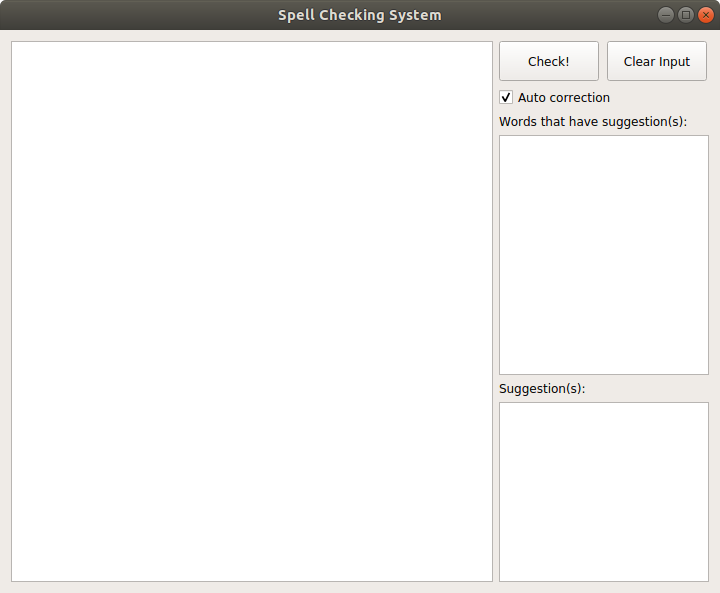
\includegraphics[width=\linewidth]{fig/main-gui.png}
	\caption{Main GUI}
	\label{fig:main-gui}
\end{figure}
\item{Two different sample navigation user paths through the data exemplifying the different modes of interaction and the corresponding screenshots. }
\begin{enumerate}
	\item {A user inputs text in the input area using keyboard.}
	\begin{figure}[H]
		\centering
		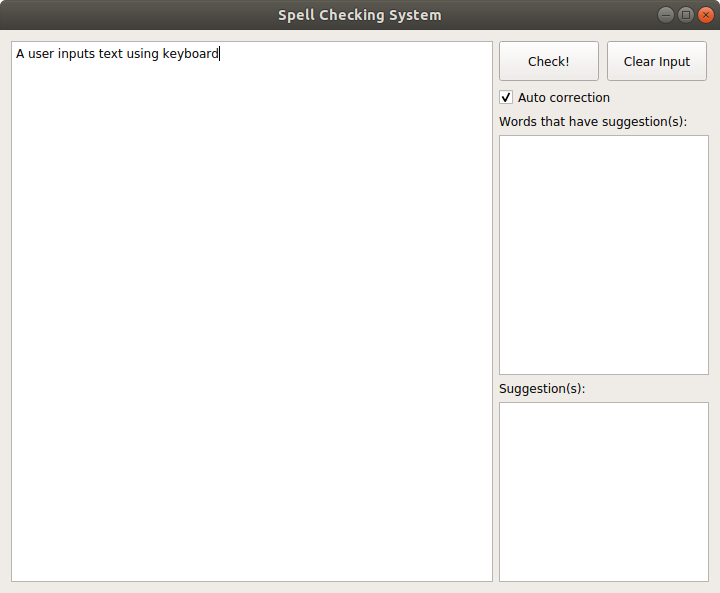
\includegraphics[width=.7\linewidth]{fig/path1.png}
	\end{figure}
	\item {A user clicks buttons or clicks items in the list using a mouse. }
	\begin{figure}[H]
		\centering
		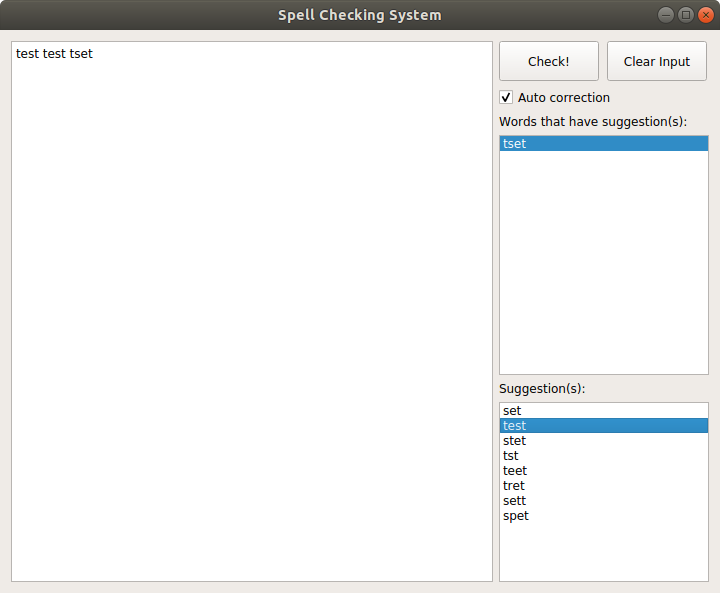
\includegraphics[width=.7\linewidth]{fig/path2.png}
	\end{figure}
\end{enumerate}
\item{}
	The error messages popping-up when users access and/or updates are denied (along with explanations and examples):
	\begin{figure}[H]
		\centering
		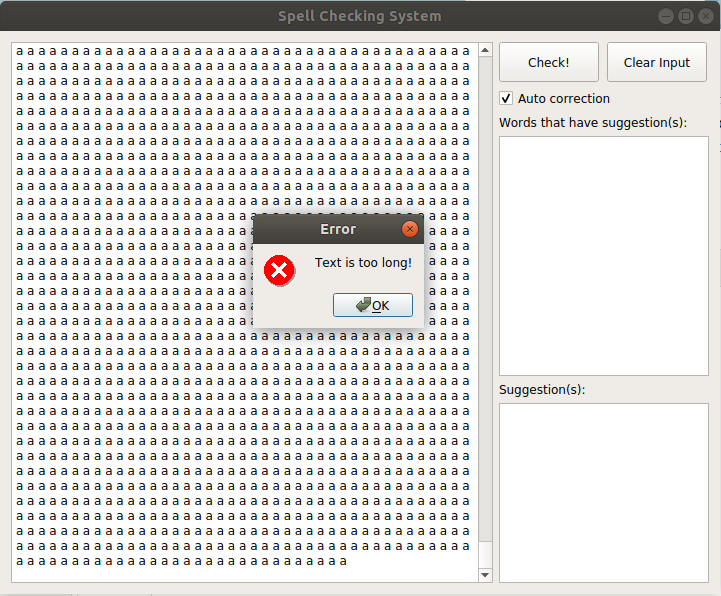
\includegraphics[width=\linewidth]{fig/error-text-too-long.png}
		\caption{Error: text is too long.}
		\label{fig:error-text-too-long}
	\end{figure}
	\begin{itemize} 
	\item{The error message: Text is too long!}
	\item{The error message explanation (upon which violation it takes place): }
	When a user tries to input more than 50,000 words in the input box, the program will pop out an error message saying that user should not input such a long text.
	\item{The error message example according to user(s) scenario(s): }
	The example is too long to be inserted here, but you can see it from the Fig \ref{fig:error-text-too-long}.
	 \end{itemize}
\item{}
	The information messages or results that pop-up in response to user interface events.
	\begin{figure}[H]
		\centering
		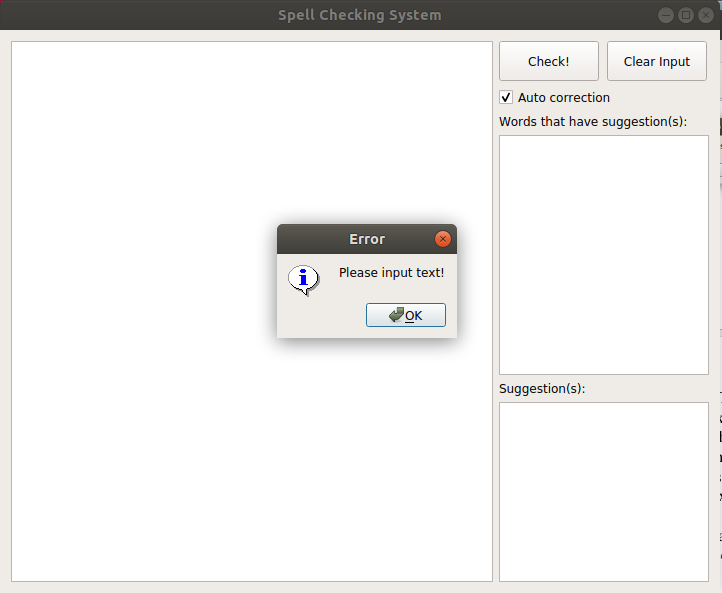
\includegraphics[width=\linewidth]{fig/info-no-text.png}
		\caption{No text inputed.}
		\label{fig:info-no-text}
	\end{figure}
	\item{The information message: Please input text!}
	\item{The information message explanation and the corresponding event trigger }
	When a user inputs nothing and click `Check' button, the program will pop out a message telling the user should input something.
	\item{The error message example in response to data range constraints and the coresponding user's scenario }
	\begin{figure}[H]
		\centering
		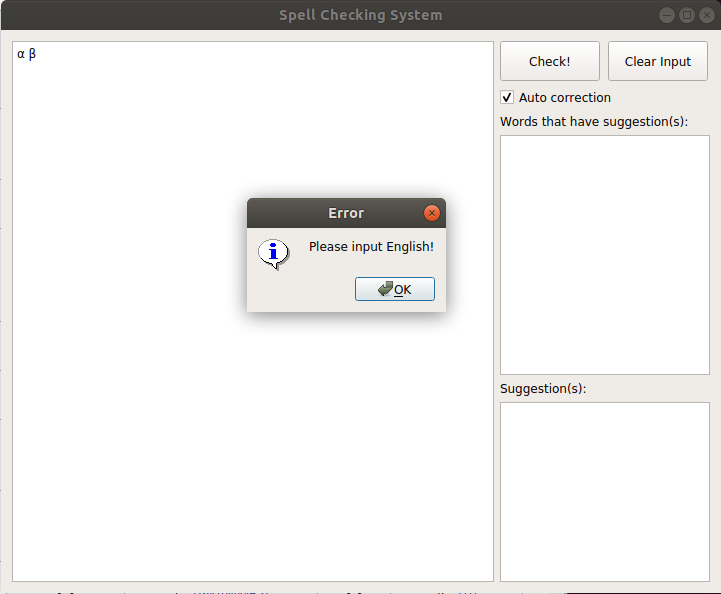
\includegraphics[width=\linewidth]{fig/eng.png}
		\caption{Please input English!}
		\label{fig:eng}
	\end{figure}
	When a user inputs non-English characters, the program will pop out a message telling the user should input English characters.
	 \end{itemize}
	The  interface mechanisms that activate different views.
	\begin{itemize} 
	\item{The interface mechanism: }
	After the main interface launches, users can input text in the input area and click buttons. If a user clicks the `check' button, the program checks if the user's input is valid. If it is valid, the program would try to find errors in the text. If the program found some errors, it would add suggestions into the `Words that have suggestion(s)' list and `Suggestion(s)' list. If a user double-clicks any item in the `Words that have suggestion(s)' list, the program would add suggestions to the `Suggestion(s)' list. If a user double-clicks any item in the `Suggestion(s)' list, the text will be corrected by this action. If a user clicks `Clear Input' button, the input area and both lists will be cleared.
	 \end{itemize}

